% Metódy inžinierskej práce

\documentclass[10pt,twoside,slovak,a4paper]{article}

\usepackage[slovak]{babel}
%\usepackage[T1]{fontenc}
\usepackage[IL2]{fontenc} % lepšia sadzba písmena Ľ než v T1
\usepackage[utf8]{inputenc}
\usepackage{graphicx}
\usepackage{url} % príkaz \url na formátovanie URL
\usepackage{hyperref} % odkazy v texte budú aktívne (pri niektorých triedach dokumentov spôsobuje posun textu)

\usepackage{cite}
%\usepackage{times}



\title{Herné umenie\thanks{Semestrálny projekt v predmete Metódy inžinierskej práce, ak. rok 2022/23, vedenie: Meno Priezvisko}} % meno a priezvisko vyučujúceho na cvičeniach

\author{Marek Fiľo\\[2pt]
	{\small Slovenská technická univerzita v Bratislave}\\
	{\small Fakulta informatiky a informačných technológií}\\
	{\small \texttt{xfilo@stuba.sk}}
	}

\date{\small 30. september 2022} % upravte



\begin{document}

\maketitle

\begin{abstract}
\ldots
\end{abstract}



\section{Úvod}

V tomto článku sa dozviete niečo málo o hernom umení, jeho umelcoch a častiach, na ktoré sa delí. Definíciu herného umenia a taktiež čo podmienilo jeho vznik sa dozviete v časti~\ref{začiatok}. Kto vytvára takéto umenie a ako začať kariéru v tomto odbore je vysvetlené v časti~\ref{pokračovanie}.





\section{Čo je to herné umenie?} \label{začiatok}
Vznik herného umenia ako ho poznáme dnes podmienil vznik počítačov a ic rozšírenie medzi širokú verejnosť.
Pod slovným spojením  \emph{Herné umenie} si môže niekto predstaviť perfektne zahranú hru či už šachu alebo niektorej z moderných počítačových hier. My pod týmto názvom rozumieme vizuálne prevedenie hry. Všetko čo vidíme na obrazovke alebo aj na našom stole je výsledkom práce herných umelcov, ktorých úlohou bolo vytvoriť návrhy a konečné prevedenia toho čo vidíme, tak aby sa to hodilo k téme hry, časovému obdobiu v ktorom sa hra odohráva a taktiež aj žánru hry.














\section{Herný umelec} \label{pokračovanie}
Herný umelec je človek, ktorý ma na svedomí vzhľad prostredia, postáv a všetkých ostatných prvkov, ktoré sa v hre vyskytujú. Umelcov rozdeľujeme na nasledovné kategórie.
\paragraph{Koncepčný umelec} Dáva základnú podobu v 2D všetkému čo sa v hre vyskytuje. S jeho návrhmi pracujú ostatný umelci a dávajú im finálnu podobu.

\paragraph{Umelec prostredia} Vytvára prostredie, modeluje 3D modely prvkov, ktoré sa v ňom nachádzajú napr. strom, dom.

\paragraph{Charakterový umelec} Výtvára vzhľad postáv.
\paragraph{Animátor postáv} Špeciálny typ 3D animátora, ktorý vdychuje život postavám.
\paragraph{FX animátor}Je zodpovedný za všetky špeciálne efekty ako napríklad výbuchy, oheň a mnohé iné. Jeho úlohou je aby tieto efekty vyzerali reálne a divák si nemyslel že sú počítačivo generované.

\section{Ako sa stať herným umelcom}
Herné umenie ako každé iné si vyžaduje kreativitu a kúsok talentu. Najprv sa treba zamerať na základy ako sú kreslenie, perspektíva, tieňovanie a hĺbka. Neodmysliteľnou súčasťou je práve kreslenie, treba sa v ňom zlepšovať a cvičiť najlepšie každý deň. Ďalším krokom je práca s programami na tvorbu grafiky, prit výbere programu, v ktorom budete pracovať záleží na tom či chcete tvoriť 2D alebo 3D grafiku. Jeden z najznámejších porgramov pre 2D grafiku je Adobe Photoshop, pre 3D grafiku to je Maya a 3DS Max, ktoré sú používané mnohými spoločnosťami.
\section{Ukážka grafických programov}

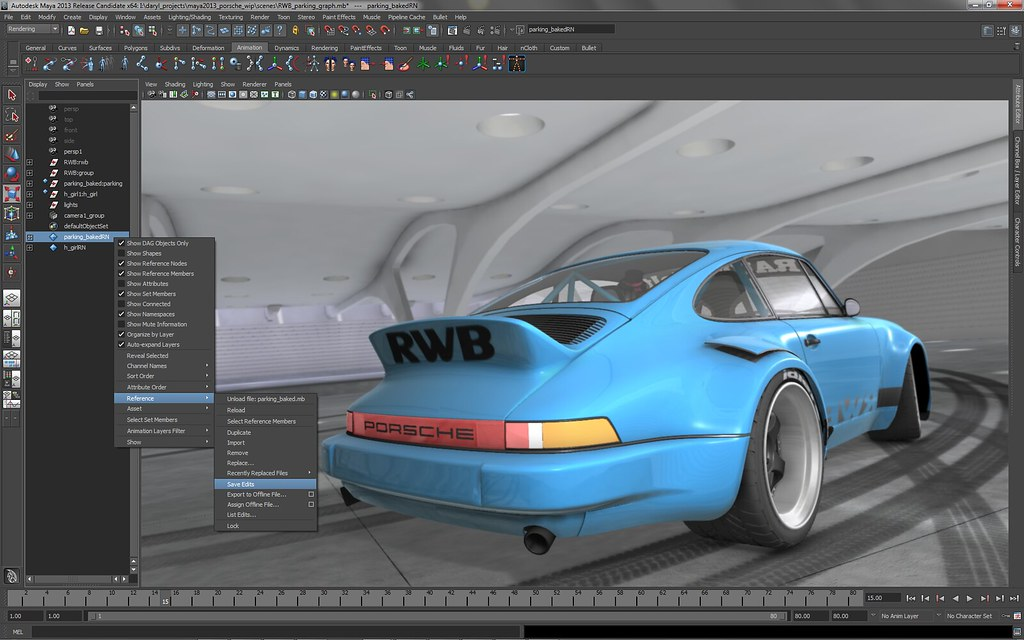
\includegraphics[width=7cm]{maya.jpg}
\caption{Maya}

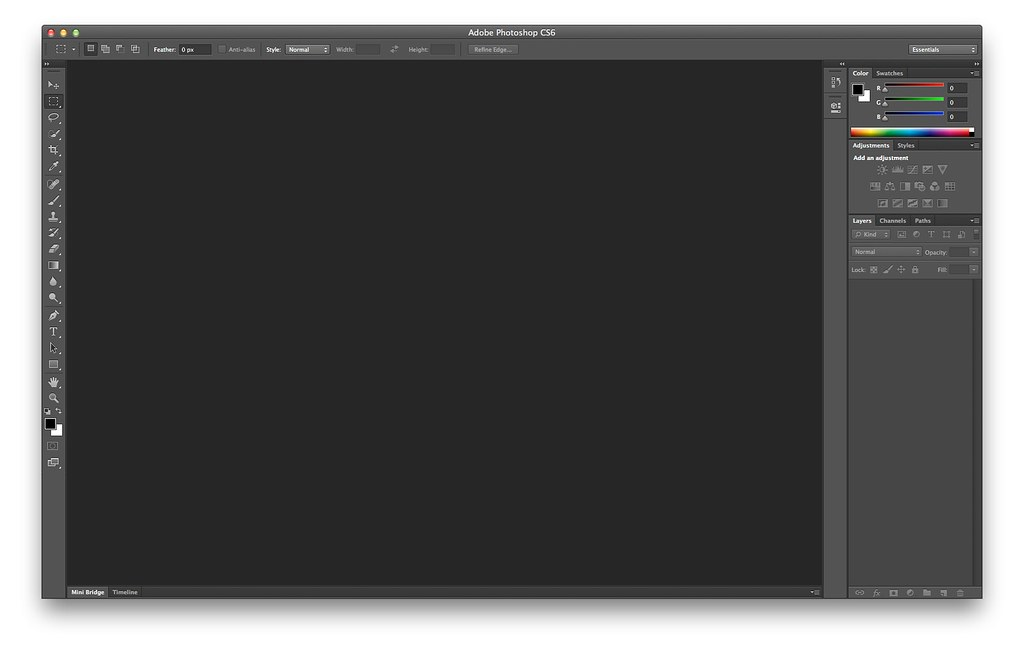
\includegraphics[width=7cm]{7006111691_df16f22507_b}
\caption{Adobe Photoshop}

\section{2D štýly herného umenia}
\paragraph{Pixel art}
Jeden z najpopulárnejších štýlov 2D. Mnoho ľudí si Pixel art spája s prvými videohrami ale tento šlýl má slušné zastúpenie aj v tejto dobe. 

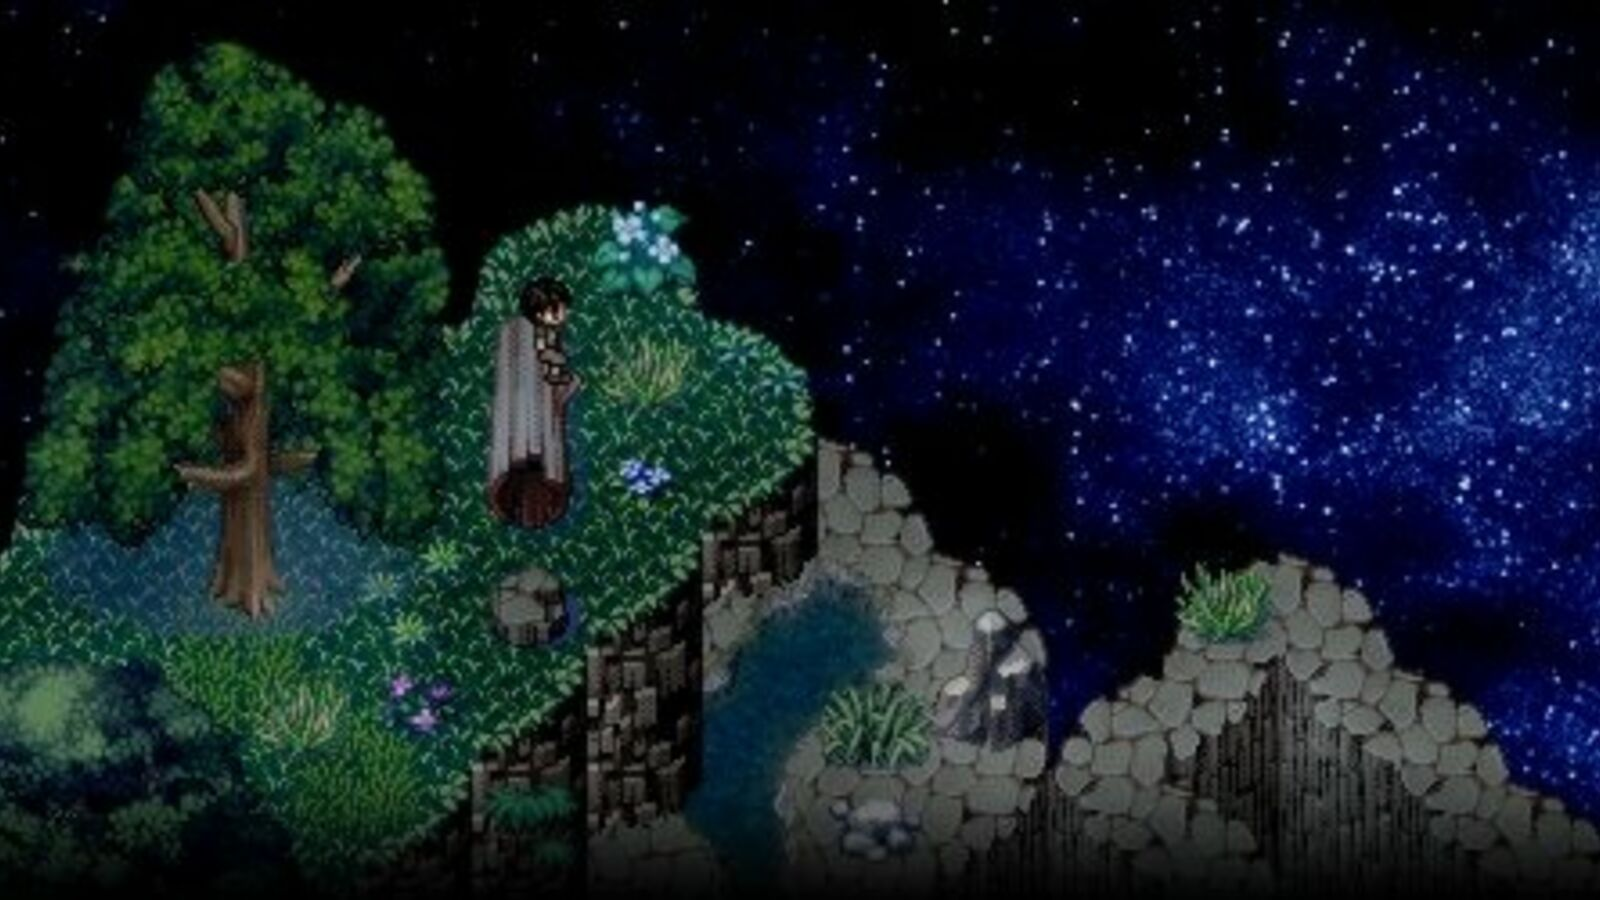
\includegraphics[width=7cm]{moon.jpg}
\caption{To the Moon} 

\paragraph{Vector art}
Ako už z názvu vyplýva v tomto štýle sa pracuje s vektorovými obrázkami. Obrázky sa nerozdeľujú na jednotlivé pixely ale ukladá ich pomocou geometrických tvarov. Výhodou je menšia veľkosť obrázkov a jedinečný vzhľad hry.




























%\acknowledgement{Ak niekomu chcete poďakovať\ldots}


% týmto sa generuje zoznam literatúry z obsahu súboru literatura.bib podľa toho, na čo sa v článku odkazujete
\bibliography{literatura}
\bibliographystyle{abbrv} % pabbrvrípadne alpha, abbrv alebo hociktorý iný
\end{document}
